\documentclass{llncs}
\usepackage{amssymb}
\usepackage{url}
\usepackage{graphicx}

%%%%%%%%%%%%%%%%%%%%%%%%%%%%%%%%%%%%%%%%%%%%%%%%%%%%%%%%%%%%%%%%%%%%%%%%%
% nastaveni stranky                                                     %
%%%%%%%%%%%%%%%%%%%%%%%%%%%%%%%%%%%%%%%%%%%%%%%%%%%%%%%%%%%%%%%%%%%%%%%%%
\setlength{\paperheight}{297mm}
\setlength{\paperwidth}{210mm}
\setlength{\textheight}{235mm}
\setlength{\textwidth}{152mm}
\setlength{\topmargin}{-25.4mm}
\setlength{\headheight}{27mm}
\setlength{\headsep}{0mm}
\setlength{\evensidemargin}{1.6mm}
\setlength{\oddsidemargin}{1.6mm}


\hyphenation{op-tical net-works semi-conduc-tor IEEEtran}


\begin{document}

\font\bigrm = cmr10 scaled \magstep 3
\font\bigmat = cmmi10 scaled \magstep 3

\font\bigrm = cmr10 scaled \magstep 3
\font\bigmat = cmmi10 scaled \magstep 3

\noindent
MUNDUS SYMBOLICUS 15 (2007)     %"��slo" ("rok")
\vskip 4 mm\noindent
\hrule
\vskip 4 mm
\centerline{\bigrm
History and Future Development of the Ferda System
}

\vskip 5 mm
\centerline{\bf
Martin Ralbovsk\'{y}
}

\vskip 4 mm
\hrule
\vskip 15 mm

\begin{abstract}
Ferda data mining system is the newest implementation of the GUHA method and has been in development for four years. The paper summarizes the history of the project and names the important student works that contributed to the project, some of which were later transformed to published papers. In addition, key directions of future development are stated.
\end{abstract}

\section{Introduction}
\label{section:introduction}
In mid-sixties, the development of the GUHA method started in Prague. GUHA is one of the first methods of exploratory data analysis and provides a general mainframe for retrieving interesting knowledge from data. The method has firm theoretical foundations based on observational calculi and statistics \cite{GUHA1,GUHA2}. Nowadays, it is used mainly for generalized association rules mining \cite{Alternative,Ra:05A,Ralbovsky}.

Over the history, the method has been several times implemented. The most significant implementation in recent history is the \emph{LISp-Miner} system, which started in 1996 at the Department of Information and Knowledge Engineering\footnote{See \url{http://lispminer.vse.cz}.}. The system contributed greatly to the level of contemporary
GUHA tools by implementing six GUHA procedures \cite{Simunek,sewebar}. However, the dialog based user environment seemed to be hard to comprehend for non-experts. 

Therefore Jan Rauch started an initiative to create a new visual user interface for \emph{LISp-Miner}. At the end of 2003, he began to lead a group of four students from the Faculty of Mathematics and Physics at Charles University, Prague with their student project, which was later named Ferda\footnote{Download at \url{http://ferda.sourceforge.net}}. Since then, a complex modular data mining system has been developed. Ferda has become an implementation platform for bachelor and master theses for students. Some of these works were scientifically important and their ideas led to published papers. These facts are little known among the scientists in the area. 

The aim of this paper is hence to present development of the system in historical context along with acknowledgment of main contributors of parts of the system and also to give a brief overview of future development. 

The paper is structured as follows: section \ref{section:features} briefly describes three main features of the system. Section \ref{section:history} describes historical making of Ferda. Section \ref{section:development} shows plans for the near future and section \ref{section:conclusion} concludes the paper. 

\section{Ferda features}
\label{section:features}
Full overview of the system was presented in \cite{Ferda}. We shall emphasis only on three key features: visualization, modularity and GUHA-ability.

\subsection{Visualization}
Ferda is visual. User builds tasks by connecting and setting visual elements at the desktop of the integrated environment, as can be seen on figure \ref{fig:Ferda}. The visual elements are called \emph{boxes} and represent abstraction of a functions. User can manipulate with boxes using other components of the environment such as archive and network archive of boxes. More details can be found in \cite{Ferda}.

\begin{figure}[ht]
\centering
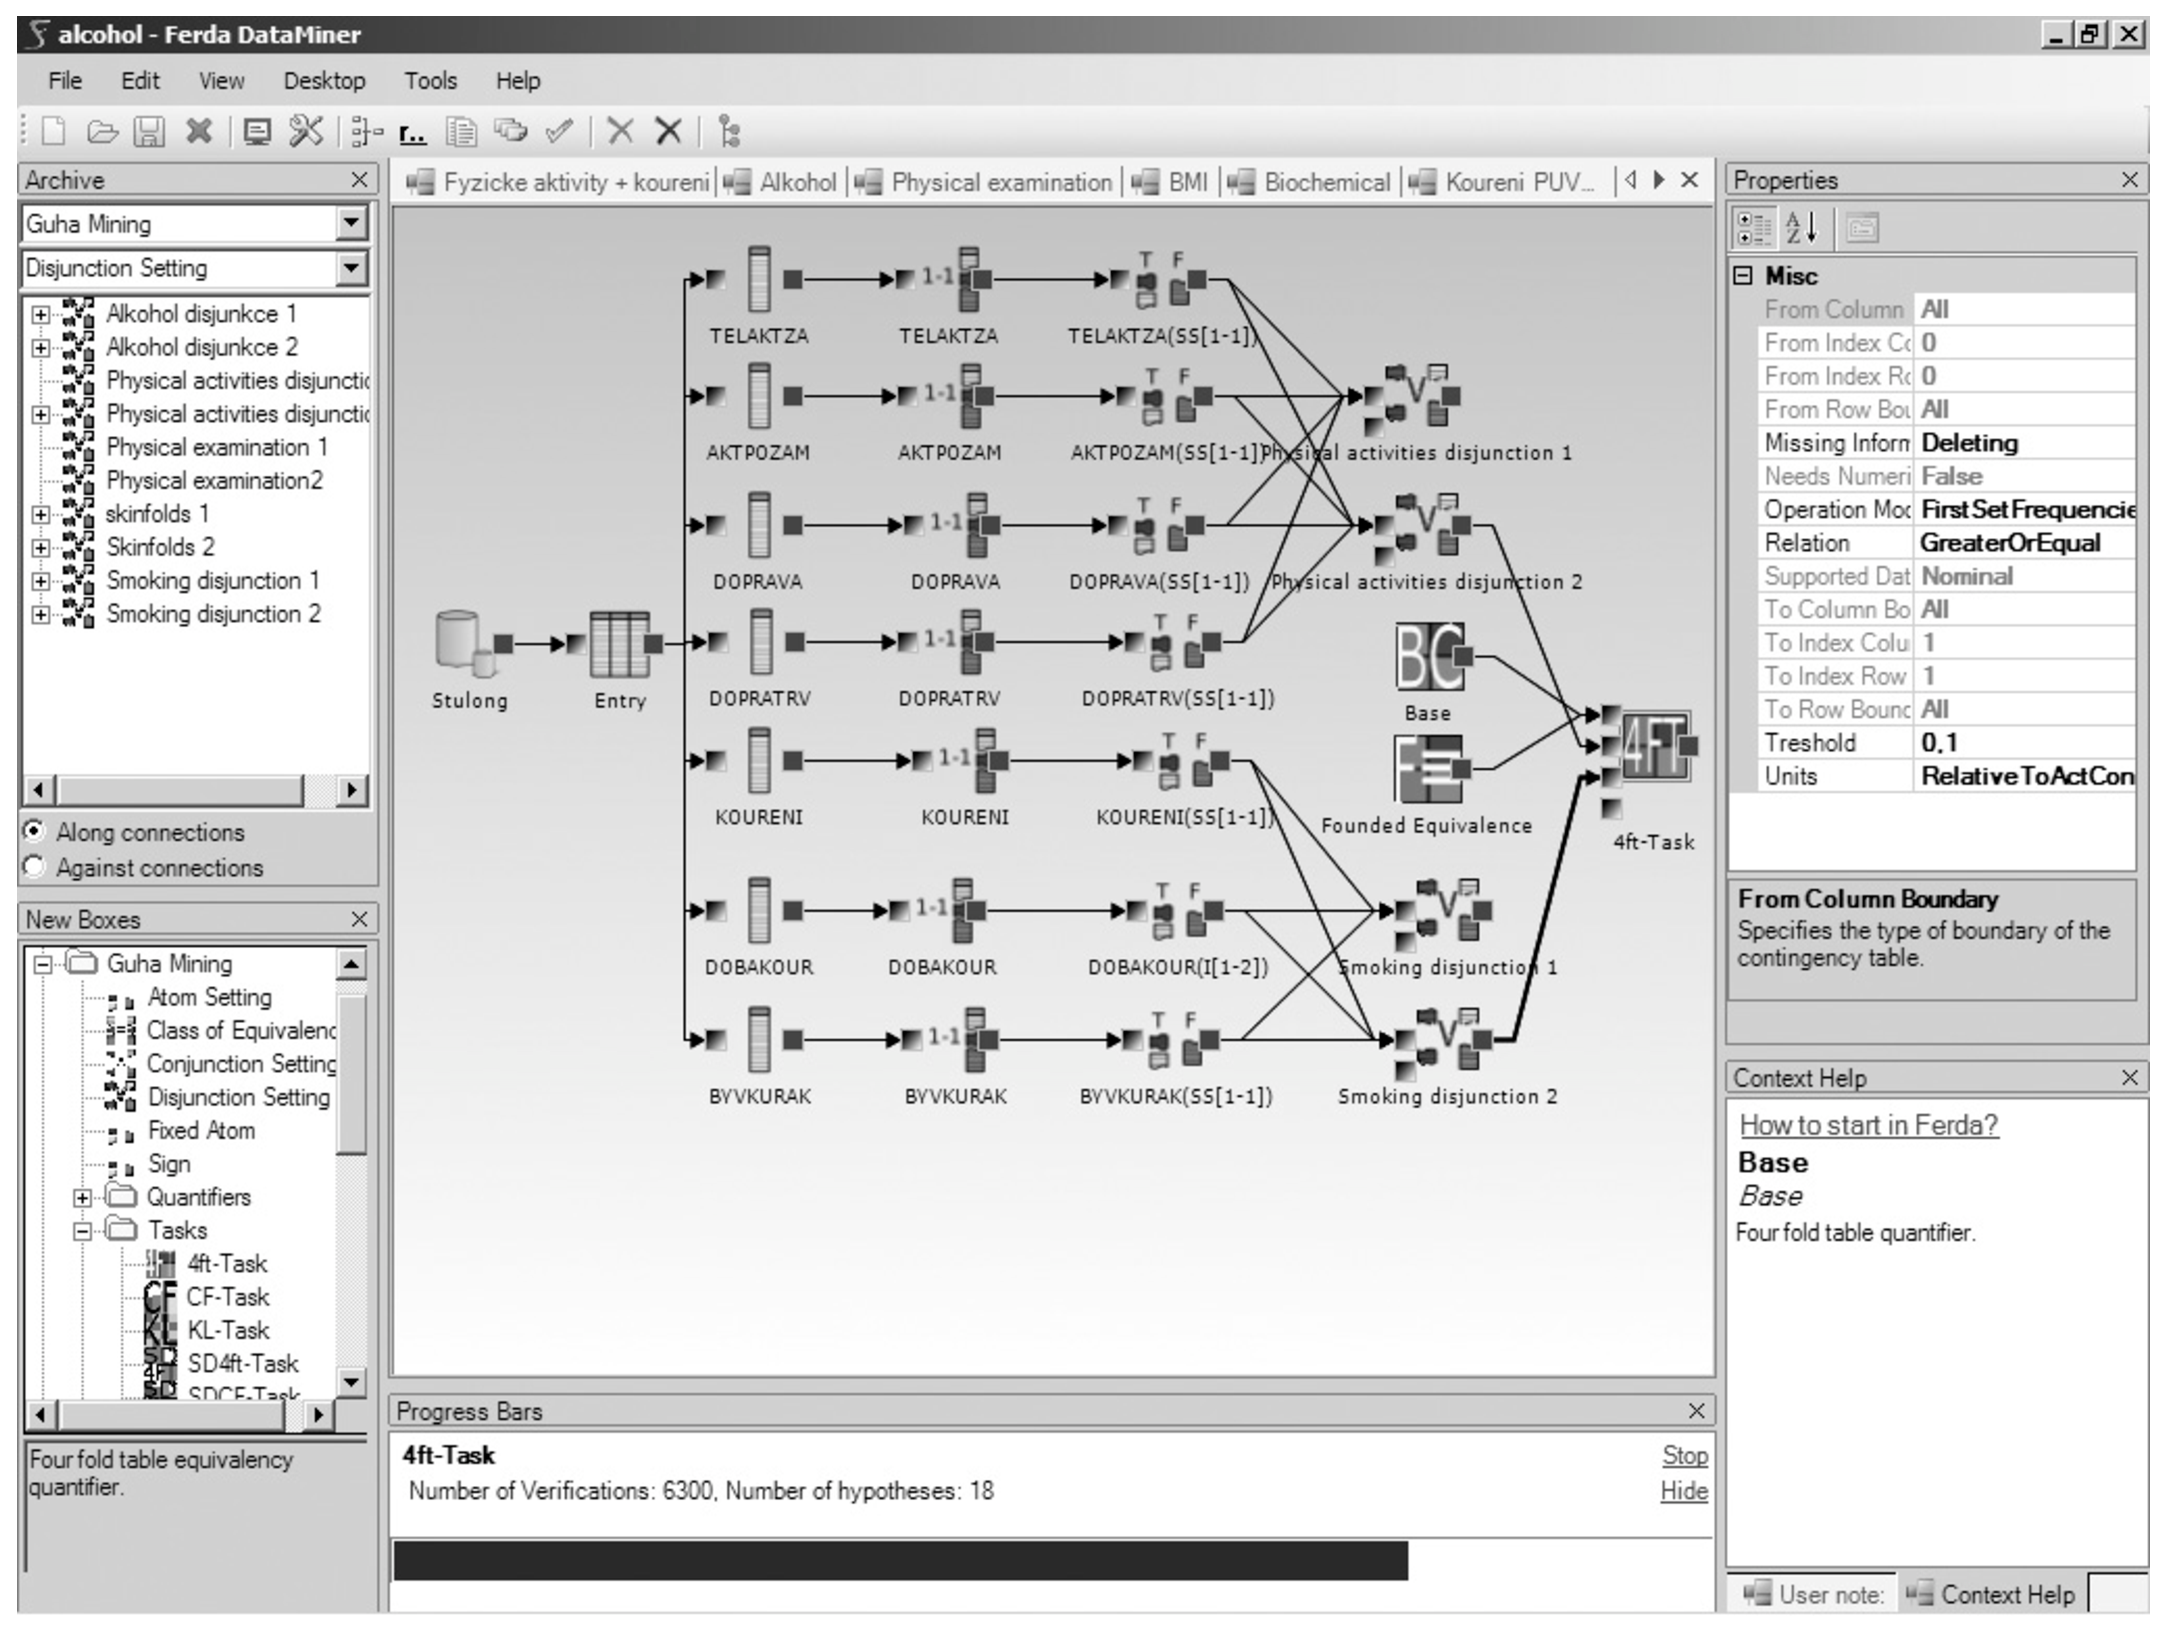
\includegraphics[width=145mm]{Ferda.eps}
\caption{Ferda environment}
\label{fig:Ferda}
\end{figure}

\subsection{Modularity}
Ferda is modular. The program runs on Ice middleware layer\footnote{\url{http://www.zeroc.com}}, which supports multiplatform communication of Ferda modules over the network. Boxes (among others) are also modules of the Ferda system. They can be written in different languages and easily added to the system. Modularity of Ferda is introduced in \cite{Ferda}, more details are to be found in system's documentation. 

\subsection{GUHA-ability}
Ferda is GUHA-able. It is a new implementation of six GUHA procedures from the \emph{LISp-Miner} system and two multirelational GUHA procedures\cite{Kuzmin}. Ferda is the first implementation of the GUHA method to enable construction of \emph{Boolean attributes} \cite{Ralbovsky}.

\section{Historical overview}
\label{section:history}

\subsection{Students' project}
History of the system began in late 2003 when Tom\'{a}\v{s} Karban introduced Jan Rauch's vision of a new visual system at presentations of student projects proposals at the Faculty of Mathematics and Physics\footnote{Students at this institution are obliged to form groups of 4 to 6 person and to develop a major software project in course of two to three years}. Students Martin Ralbovsk\'{y}, Tom\'{a}\v{s} Kucha\v{r}, Michal Kov\'{a}\v{c} and Alexander Kuzmin agreed
to apply for this project. 

In 2004, the team spent most of their time finishing other student duties and the project did not get enough priority. Real development of the system began in 2005. In spring, team made important decisions about the system architecture, middleware usage, user environment and specifications of individual boxes. Programming began in late spring and by the end of summer, individual parts of system were interconnected. In autumn, system was capable of computing first
GUHA tasks. 

In February of 2006, the system was presented at Znalosti conference with the paper \cite{Ferda}. Throughout the winter and spring, authors continued their effort to debug and optimize all parts of the system. In April, the version 1.0 of the project was acknowledged by an expert commission at the Faculty of Mathematics and Physics and the creators passed the subject. At this point, students abandon majority of the promising student projects. However, creators of Ferda decided to continue developing Ferda by choosing the system as implementation platform for their master theses. 

\subsection{Students' theses}
Martin Ralbovsk\'{y} and Tom\'{a}\v{s} Kucha\v{r} were first two to complete their master theses. They both finished in September 2006. In \cite{Diplomka}, Martin Ralbovsk\'{y} examined usage of two types of domain knowledge: ontologies and background knowledge in GUHA mining. Concerning ontologies, author enriched contemporary knowledge (mainly \cite{Cespivova1,Cespivova2}) with implementation and automation details. Thoughts from this part of the thesis were used in \cite{Ontology}. Because of the complexity of the task, the proposed processes were not implemented. Concerning background knowledge, a formalization of background knowledge was invented and a validation tool of background knowledge rules against the output of GUHA procedures was implemented in Ferda 1.0. The work (enriched by more experiments) was published in \cite{Ralbovsky2}.

The work of Tom\'{a}\v{s} Kucha\v{r} \cite{Kuchar} was motivated by problems encountered in the first version of Ferda. It used the metabase and generation libraries of the \emph{LISp-Miner} system, which caused problems with error propagation and performance. Tom\'{a}\v{s} created a new version (2.0) that implemented \emph{LISp-Miner}'s GUHA procedures with full ability of constructing \emph{Boolean attributes}. This version is significant, because it made Ferda the first KDD tool in history to mine for association rules containing \emph{Boolean attributes}. Paper \cite{Ralbovsky} is a continuation of \cite{Kuchar} and shows that these rules can be meaningful.
\medskip

Third original creator, Alexander Kuzmin finished his master thesis in June 2007. His work consisted of implementing multirelational extensions of 4FT and SD4FT procedures to the Ferda system. Computing GUHA hypotheses over multiple tables as defined in \cite{Rauch3,Karban} is a complex task. Two implementations of multirelational GUHA were carried out in the past; first one in the \emph{LISp-Miner} system and second one in unfinished PhD. work of Tom\'{a}\v{s}
Karban. Although functional, these systems were not presented to a broader scientific audience and are not used at present. Modular Ferda system made it easy for Alexander Kuzmin to implement multirelational procedures. His implementation has the advantage of visual environment, where user can better understand the complex multirelational task setting. 
\medskip

Daniel Kupka was another student from Faculty of Mathematics and Physics besides the original team, which chose Ferda as implementation platform for his master thesis. In his work \cite{Kupka} he examined one of \emph{LISp-Miner}'s GUHA procedures, \emph{4ft-miner}, in terms of user support. Thesis consists of several parts including throughout semantic analysis of \emph{4ft-quantifiers}, definition of two new quantifiers and implementation of two systems. Ferda was used for implementation of new quantifiers and as platform for one of the systems, \emph{FerdaWizard}. The thesis was completed in September 2007.
\medskip

Martin Moulis is a student of Faculty of Informatics and Statistics contributing to the project. The aim of his bachelors thesis \cite{Moulis} was to test the Ferda 2.0 implementation of the 4FT procedure against the \emph{4ft-miner} in \emph{LISp-Miner}. The work is valuable for performance comparison of the systems. Both systems gave the same results. As expected, Ferda proved to be slower then \emph{LISp-Miner}\footnote{This is mainly caused by technology used in both systems. Ferda uses middleware for communication between modules, moreover it stands on Microsoft .NET Framework. \emph{LISp-Miner} is a precompiled C++ system.}. However, in special cases the performance gap was alarming. \cite{Moulis} thus reveals optimizing problems of the Ferda system that will be dealt in the future. The thesis was also completed in 2007.
\medskip

There are two other master theses currently being processed which use Ferda. The first is work of Michal Kov\'{a}\v{c}, one of creators of the system. In addition to functional data mining boxes, Ferda contains boxes that help user to work with the functional boxes\footnote{For example the group box enables to group boxes and treat them in common.}. The main goal of Michal's thesis is to enable fully recursive programing of boxes by creating boxes for $\lambda$ abstraction, iterators or arrays. 

The second master thesis is by Martin Zeman, student of Faculty of Mathematics and Physics. His aim is to implement means of ontology support designed in \cite{Ralbovsky2}. The work uses OWL ontologies and implements boxes for ontology import into Ferda, mapping ontology terms with terms of the data source and ontology-driven creation of attributes.

\section{Future development}
\label{section:development}
As previous section showed, Ferda has been an open and modular environment suitable as implementation platform for various types of applications, mainly concerning data mining. Future development of the system goes along these lines. Currently, the system is being cofunded by the project MSM6138439910 of the Ministry of Education of the Czech Republic. The funding should provide resources for maintenance of Ferda as well as for experimental scientific research carried out with use of the system.

Nonetheless, important part of future development of Ferda are dissertations of two creators of the system, Martin Ralbovsk\'{y} and Alexander Kuzmin, who are currently studying doctoral studies at the Faculty of Informatics and Statistics. Martin Ralbovsk\'{y} aims to implement fuzzy extensions of GUHA procedures \cite{Fuzzy} implemented in Ferda, mainly by enabling fuzzy bit strings and fuzzy quantifiers. Alexander Kuzmin will be investigating multirelational GUHA hypotheses in terms of usability and comprehensibility.

There is an ongoing initiative by Faculty of Informatics and Statisticks PhD. student Tom\'{a}\v{s} Kliegr dubbed GAIN to extend the work presented in \cite{EKAW}, whose goal is to use Ferda as a common platform for streamlining web usage mining tasks. Ferda's built-in features can be used to connect directly to clickstream data mart. The GAIN-CL and GAIN-DR box should apply clickstream-specific data cleansing and dimension reduction tasks.

Apart from the above mentioned planned activities, there are suggestions to implement GUHA-like decision trees, classification algorithms and proving in special kinds of logics.

\section{Conclusion}
\label{section:conclusion}
Ferda system for (not only) GUHA mining is in fourth year of existence. The paper maps history of the project from early stages of a student project to stage of a modular and visual implementation platform of many promising student works, many of which served as basis for scientific publications. The paper also states important features of the project as well as lookup for future development. 

\subsection*{Acknowledgments}
This work was supported by the project MSM6138439910 of the
Ministry of Education of the Czech Republic, project IG407056 of University
of Economics, Prague and by the project 201/05/0325 of the Czech Science
Foundation. I would like to thank Jan Rauch for wise advices and supervision of the project, members of the original Ferda team and also to all the remaining contributors. 

\begin{thebibliography}{20}

\bibitem{Cespivova1}
\v{C}E\v{S}PIVOV\'{A} H.: Creation of Ontologies for Knowledge Discovery in Databases. 
Master Thesis, Faculty of Informatics and Statistics, University of Economics, Prague 2004 (in Czech)

\bibitem{Cespivova2}
\v{C}E\v{S}PIVOV\'{A} H., RAUCH J., SV\'{A}TEK V., KEJKULA M., TOME\v{C}KOVA M.:
Roles of Medical Ontology in Association Mining CRISP-DM Cycle. ECML/PKDD04 Workshop on Knowledge Discovery and Ontologies (KDO'04), Pisa 2004

\bibitem{GUHA1}
H\'{A}JEK P., HAVEL I., CHYTIL M.: The GUHA method of
automatic hypotheses determination. Computing 1, 1966, p.~293~--~308

\bibitem{GUHA2}
H\'{A}JEK P., HAVR\'{A}NEK, T.: Mechanising Hypothesis
Formation - Mathematical  Foundations  for  a   General  Theory.
Springer-Verlag: Berlin  - Heidelberg - New York, 1978.

\bibitem{Fuzzy}
H\'{A}JEK P., HOLE\v{N}A M.: Formal logics of discovery and
hypothesis formation by machine. in Discovery Science: First International 
Conference proceedings, DS'98, Fukuoka Japan, 1998, Springer Verlag, ISSN:0302-9743

\bibitem{Karban}
KARBAN T.: Relational Data Mining and GUHA. in Richta K., 
Sn\'{a}\v{s}el V., Pokorn\'{y} J.(eds.): Proceedings of the 5th annual
workshop DATESO 2005(Databases, Texts, Specifications and Objects),
ISBN:80-01-03204-3, pp.103--112

\bibitem{EKAW}
KLIEGR T.: Clickstream analysis - the semantic approach. 
In Helena Sofia Pinto and Martin Labsk\'{y}, editors, Poster and Demo 
Proceedings of EKAW 2006 - 15th International Conference on Knowledge 
Engineering and Knowledge Management 2006. ISBN 80-86742-15-6.

\bibitem{Kovac}
KOV\'{A}\v{C} M.:User oriented language for solving KDD tasks, 
Faculty of Mathematics and Physics, Charles University, Prague (to appear)

\bibitem{Ferda}
KOV\'{A}\v{C} M., KUCHA\v{R} T., KUZMIN A., RALBOVSK\'{Y} M.: Ferda, 
New Visual Environment for Data Mining. Znalosti 2006, 
Conference on Data Mining, Hradec Kr\'{a}lov\'{e} 2006, p.~118~--~129 (in Czech)

\bibitem{Kuchar}
KUCHA\v{R} T.: Experimental GUHA Procedures, Master Thesis, 
Faculty of Mathematics and Physics, Charles University, Prague 2006 (in Czech)

\bibitem{Kupka}
KUPKA D.: User support 4ft-miner procedure for data mining. Master Thesis,
Faculty of Mathematics and Physics, Charles University, Prague 2007 (in Czech)

\bibitem{Kuzmin}
KUZMIN A.: Relational GUHA procedures. Master Thesis, 
Faculty of Mathematics and Physics, Charles University, Prague 2007 (in Czech)

\bibitem{Moulis}
MOULIS. M.: Testov\'{a}n\'{i} softwarov\'{e}ho syst\'{e}mu Ferda.
Bachelors Thesis, Faculty of Informatics and Statistics, University of Economics,
Prague 2007 (in Czech)

\bibitem{Ralbovsky2}
RALBOVSK\'{Y} M.: Evaluation of GUHA Mining with Background Knowledge. ECML/PKDD07 Workshop on Prior Conceptual Knowledge in Machine Learning and Knowledge Discovery (PriCKL'07), Warsaw 2007

\bibitem{Diplomka}
RALBOVSK\'{Y} M.: Usage of Domain Knowledge for Applications of GUHA
Procedures, Master Thesis, Faculty of Mathematics and Physics, Charles University,
Prague 2006 (in Czech)

\bibitem{Ralbovsky}
RALBOVSK\'{Y} M., KUCHA\v{R} T.: 
Using Disjunctions in Association Mining. 
In: P. Perner (Ed.),
Advances in Data Mining - Theoretical Aspects and Applications, LNAI
4597, Springer Verlag, Heidelberg 2007

\bibitem{Ra:05A}
RAUCH J.:Logic of Association Rules. Applied Intelligence,
 22, pp. 9 - 28, 2005

\bibitem{Rauch3}
RAUCH J.: Many Sorted Observational Calculi for Multi-Relational Data Mining.
In: Data Mining � Workshops. Piscataway: IEEE Computer Society, 2006 
ISBN 0-7695-2702-7 p.~417--422

\bibitem{Alternative}
RAUCH J., \v{S}im\accent23unek, M.: An Alternative Approach to Mining
Association Rules. Lin T Y, Ohsuga S, Liau C J, and Tsumoto S (eds):
Foundations of Data Mining and Knowledge Discovery, Springer-Verlag, 2005
p.~219~--~239

\bibitem{sewebar}
RAUCH J., \v{S}im\accent23unek, M.: Dealing with Background Knowledge in the SEWEBAR Project. ECML/PKDD07 Workshop on Prior Conceptual Knowledge in Machine Learning and Knowledge Discovery (PriCKL'07), Warsaw 2007

\bibitem {Simunek}
\v{S}IM\accent23UNEK M.: Academic KDD Project LISp-Miner.
In Abraham A. et al (eds): Advances in Soft
Computing - Intelligent Systems Design and Applications, 
Springer Verlag 2003

\bibitem{Ontology}
SV\'{A}TEK V., RAUCH J., RALBOVSK\'{Y} M.: Ontology-Enhanced Association
Mining. In: Ackermann, Berendt (eds.). Semantics, Web and Mining, 
Springer-Verlag, 2006
\end{thebibliography}

\bigskip
\bigskip
\noindent
Department of Information and Knowledge Engineering,\\
Martin Ralbovsk\'{y}  \\
Faculty of Informatics and Statistics \\ 
University of Economics, Prague  \\
n\'{a}m W. Churchilla~4,\\
130 67 Prague, 
Czech Republic,\\
\email{martin.ralbovsky@gmail.com}


\end{document}